\documentclass{beamer}

\setbeamertemplate{bibliography item}{[\theenumiv]}

\usetheme{Madrid}
%\usecolortheme{seahorse}
\usepackage[brazil]{babel}
\usepackage[utf8x]{inputenc} % acentos diretamente do teclado
\usepackage[T1]{fontenc}
\usepackage{graphicx}
\usepackage{xcolor}
\usepackage{listings}
%\usepackage{courier}
\usepackage[scaled=0.8]{beramono}


\title[Programação Paralela]{Intel Cilk Plus}
\subtitle{Programação Paralela}
\author[Alexandre \and Jeremias \and Matheus]{Alexandre Lucchesi%
    \and Jeremias Moreira%
    \and Matheus Braga}
\institute[UnB]{%
    Departamento de Ciência da Computação\\
    Universidade de Brasília, Brasília -- DF\\[1ex]
    \texttt{alexandrelucchesi@gmail.com}\\
    \texttt{jeremias@aluno.unb.br}\\
    \texttt{matheus.mtb7@gmail.com}\\
}
\date[Outubro, 2014]{10 de outubro de 2014}


\lstset{%
    language=C,
    basicstyle=\ttfamily,
    breaklines=true,
    morekeywords={cilk\_for, cilk\_spawn, cilk\_sync, cilk, grainsize}
}


\begin{document}

\begin{frame}[plain]
    \titlepage%
\end{frame}

\begin{frame}[shrink]{Sumário}
    \tableofcontents
\end{frame}


%\section{Introdução}
%\subsection{O que é}
%\begin{frame}{Introdução}
%    \begin{itemize}
%        \item Cilk Plus é ``dahora''~\cite{jeffers:2013}.
%    \end{itemize}
%\end{frame}

\section{História}
\begin{frame}{História do Cilk}
\begin{itemize}
    \item O MIT desenvolveu o Cilk: uma tecnologia para programação
    \textit{multithread};
    \item O Cilk generaliza a semântica do C e introduz novas construções
    sintáticas para permitir a expressão de paralelismo;
    \item \textbf{O programador} deve se concentrar em estruturar seus programas
    de forma a explorar o \textbf{paralelismo} e a \textbf{localidade};
    \item \textbf{O Cilk} deve ser responsável pelo \textbf{escalonamento de
    tarefas} (em tempo de execução) maximizando o desempenho em
    \textbf{diferentes plataformas}.
\end{itemize}
\end{frame}

\begin{frame}{História do Cilk}
\begin{itemize}
    \item Cilk-1: suporte eficiente a \textbf{\textit{work-stealing}};
    \item Cilk-5: extensões simples para \textit{multithread} em ANSI C\@;
    \item Cilk++: versão comercial para C++ que introduziu reduções de
    hiperobjetos como técnica eficiente em aplicações cuja programação é
    irregular (ex: simulações N-body, \textit{tree search}, etc);
    \item Cilk Plus: adicionou extensões para matrizes e foi incorporado ao
    compilador da Intel~\footnote{Pouco tempo após o lançamento do Cilk Plus, a
    Intel tornou pública as especificações da linguagem, permitindo sua
    incorporação em outros compiladores. Atualmente, além do compilador
    \texttt{icc}, o Cilk Plus pode ser encontrado em versões do \texttt{gcc} e
    do \texttt{clang} (de forma limitada).}.
\end{itemize}
\end{frame}

\section{Funções Principais}
\begin{frame}{Cilk Plus \textit{in a nutshell}\ldots}
\begin{itemize}
    \item Elementos básicos:
    \begin{itemize}
        \item \texttt{cilk\_for};
        \item \texttt{cilk\_spawn};
        \item \texttt{cilk\_sync}.
    \end{itemize}
    \item Redução com hiperobjetos;
    \item Notação matricial.
\end{itemize}
\end{frame}

\begin{frame}[fragile]{\texttt{cilk\_for}}
\begin{itemize}
    \item Permite que as iterações sejam executadas em paralelo.
\end{itemize}
\begin{exampleblock}{Exemplo}
\begin{lstlisting}
void saxpy(float a, float x[], float y[], size_t n) {
    cilk_for (size_t i = 0; i < n; i++)
        y[i] += a * x[i];
}
\end{lstlisting}
\end{exampleblock}
\end{frame}

\begin{frame}[fragile]{\texttt{cilk\_for}}
\begin{columns}[T]
\begin{column}{0.5\textwidth}
\begin{itemize}
    \item A sintaxe do \texttt{cilk\_for} tem algumas limitações, pois deve ser
    possível computar o espaço de iterações antes de executar o \textit{loop};
    \item O \texttt{corpo} deve ser paralelizável;
    \item O tipo de \texttt{idx} deve ser um inteiro ou \textit{iterator} de
    acesso randômico (ex: um ponteiro);
    \item Em \texttt{cond} podem ser utilizados somente: ${ !=, <, >, >=, <= }$;
\end{itemize}
\end{column}

\begin{column}{0.5\textwidth}
\begin{block}{}
\begin{lstlisting}
cilk_for(idx = expr; cond; incr)
    corpo;
\end{lstlisting}
\end{block}
\begin{itemize}
    \item \texttt{incr} é composto de um limite (\texttt{lim}) e um passo que
    devem ser avaliados apenas uma vez (imutáveis);
    \item O incremento (ou decremento) pode ser expressado com ${ +=, -=, ++,
    --}$.
\end{itemize}
\end{column}

\end{columns}
\end{frame}

\begin{frame}[fragile]{\texttt{cilk\_for}}
\begin{itemize}
    \item Por padrão, o \texttt{cilk\_for} divide (\textit{tiles}) o espaço de
    iterações: 
    \begin{itemize}
        \item As \textit{threads} executam todo o \textit{tile};
        \item Evita sincronizações excessivas.
    \end{itemize}
    \item Para casos em que é necessário maior controle acerca da granularidade,
    pode-se o utilizar o \textbf{\texttt{pragma cilk grainsize}} para
    especificar o tamanho de um \textit{tile}:
\begin{lstlisting}
#pragma cilk grainsize = 1
cilk_for (int i = 0; i < n; i++)
    a[i] = f(b[i]);
\end{lstlisting}
\end{itemize}

\end{frame}

{% Spawn's pic. ;)
\usebackgroundtemplate{
\includegraphics[width=\paperwidth,height=\paperheight]{./img/spawn.jpg}}
\begin{frame}{\texttt{cilk\_spawn}}
\end{frame}
}

\begin{frame}[fragile]{\texttt{cilk\_spawn}}
\begin{itemize}
    \item O \texttt{cilk\_spawn} cria e executa uma nova \textit{thread}
    de \textbf{forma assíncrona};
    \item Possui mecanismos que possibilitam a recuperação do valor de retorno
    da chamada assíncrona~\footnote{Os argumentos passados para a função são
    avaliados antes do \textit{fork} (\textit{strict evaluation}).}:
\begin{lstlisting}
x = cilk_spawn f(*p++);
\end{lstlisting}
    \item É possível criar chamadas assíncronas de um conjunto de instruções
    através de \textbf{expressões lambda}:
\begin{lstlisting}
cilk_spawn [&]{
    for (int i = 0; i < n; i++)
        a[i] = 0;
} ();
\end{lstlisting}
\end{itemize}
\end{frame}

\begin{frame}{\texttt{cilk\_sync}}
\begin{itemize}
    \item O \texttt{cilk\_sync} consiste em um mecanismo de sincronização que se
    assemelha a um \textit{join}.
    \item O escopo de uma chamada \texttt{cilk\_sync} é a função inteira na qual
    foi declarada e existe uma chamada \texttt{cilk\_sync} implícita no final de
    cada função.
    \item Isso implica que todo o paralelismo criado com o Cilk Plus em
    determinada função, termina antes que ela retorne.
\end{itemize}
\end{frame}

\begin{frame}[fragile]{\emph{Not only} uma questão de estilo\ldots}
\begin{columns}[c]

\begin{column}{0.3\textwidth}
\begin{block}{Código}
% Bad style...
\begin{lstlisting}
...
cilk_spawn f();
cilk_spawn g();
...
cilk_sync;
...
\end{lstlisting}
\end{block}
\end{column}

\pause

\begin{column}{0.6\textwidth}
\begin{figure}
\centering
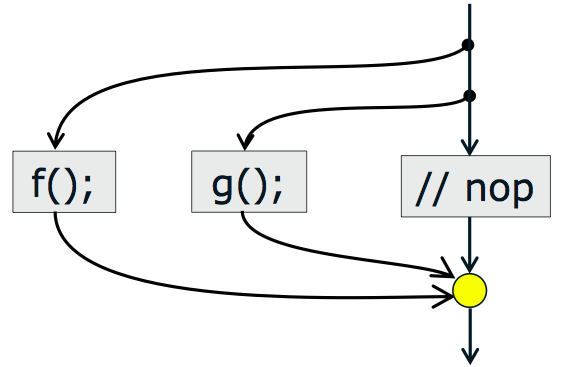
\includegraphics[width=\columnwidth]{./img/bad-style.png}
\end{figure}
\end{column}
\end{columns}
\end{frame}

\begin{frame}[fragile]{\emph{Not only} uma questão de estilo\ldots}
\begin{columns}[c]

\begin{column}{0.3\textwidth}
\begin{block}{Código}
% Good style...
\begin{lstlisting}
...
cilk_spawn f();
g();
...
cilk_sync;
...
\end{lstlisting}
\end{block}
\end{column}

\pause

\begin{column}{0.4\textwidth}
\begin{figure}
\centering
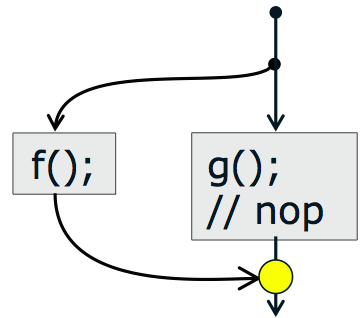
\includegraphics[width=\columnwidth]{./img/good-style.png}
\end{figure}
\end{column}
\end{columns}
\end{frame}

\begin{frame}[fragile]{\textit{Serial Elision}}
\begin{itemize}
    \item O Cilk Plus, de uma forma geral, é uma linguagem pouco intrusiva;
    \item Isso fica explícito quando se deseja, por exemplo, obter a versão
    serial (\textit{serial elision}) de um programa Cilk Plus: basta eliminar as
    palavras-chave \texttt{cilk\_spawn}, \texttt{cilk\_sync} e
    \texttt{cilk\_for};
    \item De forma trivial:
\begin{lstlisting}
#define cilk_spawn
#define cilk_sync
#define cilk_for for
\end{lstlisting}
    \item O resultado é um programa serial C/C++ válido.
\end{itemize}
\end{frame}

\subsection{Exemplos}
\begin{frame}{Exemplos}
\end{frame}

\begin{frame}{Análise Comparativa}
\section{Análise Comparativa}
\subsection{Gráfico de \protect\textit{Speedup}}
\end{frame}

\section{Aspectos da Ferramenta}
\subsection{Vantagens}
\begin{frame}{Vantagens}
\begin{itemize}
    \item Diretivas básicas bem definidas e de uso trivial.
    \item Uso de uma forma de\textit{ Syntax sugar} para trabalhar com arrays.
    \item Focada em optimizar resultados em processadores da Intel\circledR.
    \item Implementa SIMD.
    \item Alto nivel e abstração, a linguagem cuida de quase tudo.  O programador nao precisa se preocupar com quase nada. Tudo ja está praticamente implementado.
\end{itemize}

\end{frame}

\subsection{Desvantagens}
\begin{frame}{Desvantagens}
\begin{itemize}
    \item Dificuldade de se intalar.
    \item Muito invasiva, necessita de modificações no compilador e faz alterações na própria sintaxe.
    \item ?
    \item Alto nivel e abstração, a linguagem cuida de quase tudo. Ou seja, para casos onde seja necessário uma optimização, vai ser bem complicado.
\end{itemize}

\end{frame}


\section{Conclusão}
\begin{frame}%[allowframebreaks]
    \frametitle{Referências Bibliográficas}
    \tiny{\bibliographystyle{abbrv}}
    \bibliography{refs}
\end{frame}

\end{document}

